%%% Local Variables:
%%% mode: latex
%%% TeX-master: "../doc"
%%% coding: utf-8
%%% End:
% !TEX TS-program = pdflatexmk
% !TEX encoding = UTF-8 Unicode
% !TEX root = ../doc.tex

3D-Visualisierungen werden in vielen Branchen verwendet. Virtual Reality, CAD-Programme oder Computerspiele sind einige bekannte Anwendungsgebiete. Dank leistungsstärkeren Geräten sind in vielen weiteren Bereichen realere Visualisierungen möglich.

Anwendungen können auf spezifische Hardware, wie zum Beispiel die Spielkonsole PlayStation, ausgerichtet sein. Es gibt Unterschiede zwischen den Konsolen, grundsätzlich sind die verschiedenen Geräte jedoch überschaubar. In anderen Anwendungsfällen kann eine Applikation sogar für nur eine dedizierte Hardware entwickelt werden. Somit kann eine Applikation auf die Anforderungen dieser Hardware zugeschnitten werden. Der primäre Nachteil ist dann die Zugänglichkeit der Software, da spezifische Hardware notwendig ist. So ist es einerseits aufwändig die Hardware zu beschaffen, andererseits aber auch eine Kostenfrage. Für gewisse Anwendungsgebiete ist dies ein zweitrangiges Problem.

Für hardwareunabhängige Anwendungen eignet sich die Web-Plattform hervorragend.
Immer mehr Benutzer haben Zugang zu einem Desktop, Tablet, Mobiltelefon oder ein anderes Gerät, welches Zugang zum Internet bietet \cite{peopleWithInternetAccess}.
Somit ermöglicht die Web-Plattform, Anwendungen mit weniger Aufwand einem grossen Zielpublikum zugänglich zu machen.
Seit einigen Jahren ist es auch möglich, 3D-Visualisierungen im Web zu realisieren.

\section{Kontext}
In der Arbeit wird der Fokus auf die Web-Plattform gelegt. Die meisten Grundlagen sind jedoch auch unabhängig davon zutreffend.
Für die Vereinfachung wird im Folgenden der Begriff Web für die Plattform von verschiedenen Web-Technologien genutzt. Dies beinhaltet insbesondere vom \e{World Wide Web Consortium}, kurz W3C, veröffentlichte Standards.

\section{Ausgangslage}
Dank der Rechenleistung auf modernen Geräten ist es möglich anspruchsvolle 3D-Visualisierungen in Echtzeit auf diversen Geräten anzuwenden. Da diese Applikationen sehr rechenintensiv sind und gerade mobile Geräte in ihrer Rechenleistung beschränkt sind, ist Performance Optimierung im 3D-Rendering unabdinglich. Insbesondere die Komplexität der Modelle hat einen signifikanten Einfluss auf die Leistung.
Eine Möglichkeit zur Optimierung ist das Anzeigen von vereinfachten Modellen ab bestimmten Distanzen zum Betrachter. So kann z.B. ein Modell in grosser Distanz vereinfacht (Abbildung \ref{fig:lodComparisonSimplified}) dargestellt werden, solange bei genauer Betrachtung mehr Details (Abbildung \ref{fig:lodComparisonOriginal}) sichtbar werden.

\begin{figure}[H]
  \centering
  \begin{subfigure}{.4\textwidth}
    \centering
    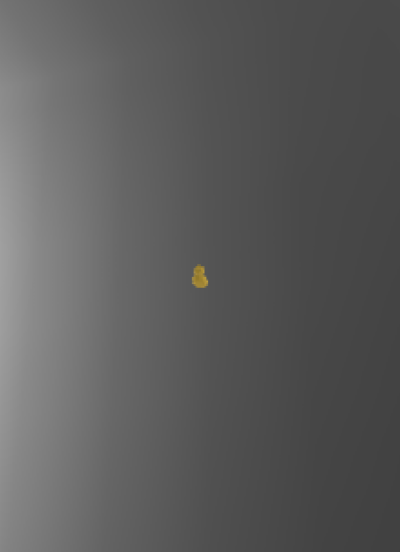
\includegraphics[width=.8\linewidth]{resultate/simplified-distance.png}
    \caption{vereinfachtes Modell entfernt}
    \label{fig:lodComparisonSimplified}
  \end{subfigure}
  \begin{subfigure}{.4\textwidth}
    \centering
    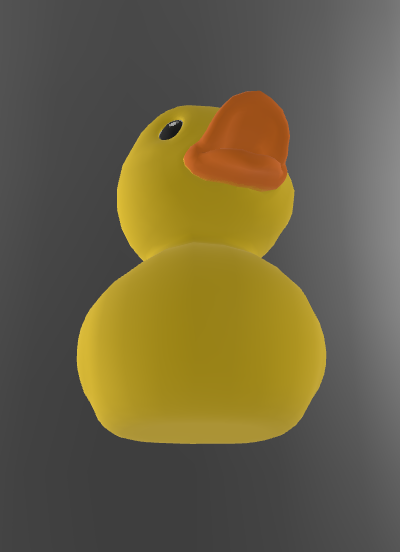
\includegraphics[width=.8\linewidth]{resultate/lod-original.png}
    \caption{Originalmodell nah}
    \label{fig:lodComparisonOriginal}
  \end{subfigure}
  \caption{Vergleich vereinfachtes Modell (entfernt) Originalmodell (nah)}
\end{figure}

In diversen \fglspl{Rendering Engine}{Teilprogramm, das zuständig für die Darstellung von Grafiken ist} gibt es deshalb Möglichkeiten für das Verwenden von sogenannten Level Of Details (LOD) Artefakten.
Für \fgls{Game Engines}{Framework, das für den Spielverlauf und dessen Darstellung verantwortlich ist} wie \e{Unreal Engine} oder \e{Unity} gibt es bewährte Möglichkeiten, um den Einsatz von LOD-Artefakten zu vereinfachen. Zurzeit gibt es in der Webentwicklung keine weitverbreitete Möglichkeit für das Generieren von solchen Artefakten.

\subsection{3D-Rendering im Web}

Als Basis für 3D-Visualisierungen im Web dient meist das von der Khronos Group entwickelte WebGL, das von allen modernen Browsern unterstützt wird. WebGL ist eine low-level JavaScript API für 3D-Visualisierungen \cite{webGl1Spec}.
Alternativ zu WebGL wird zurzeit ein weiterer Standard entwickelt: WebGPU. Dieser ist zur Zeit des Schreibens noch in Entwicklung und wird deshalb nicht weiter berücksichtigt, auch wenn ein grosses Potenzial vorhanden ist \cite{webGPUCharter}.

Die Unabhängigkeit der Hardware bedeutet jedoch auch, dass Optimierung der Performanz in Webanwendungen unabdinglich ist, um allen Benutzern ein optimales Erlebnis zu ermöglichen.
Im Vergleich zu fixen Hardware Anwendungen ist es realistisch, dass eine Webanwendung sowohl auf einem leistungsfähigen Desktop Computer als auch auf einem günstigen Mobilgerät verwendet wird.

Zudem ist WebGL eine junge Technologie und wurde erst 2011 veröffentlicht – verglichen mit dem initialen Release Date von \fgls{OpenGL}{Spezifikation einer Programmierschnittstelle zur Entwicklung von 2D- und 3D-Grafikanwendungen} welches im Jahre 1992 publiziert wurde \cite{webGl1Spec,openGlSpec}.
Nicht nur das Alter, sondern auch die Natur der Web-Plattform haben dazu beigetragen, dass WebGL ein langsames Wachstum verspürt hat. Um einen Webstandard wie WebGL einsetzen zu können, müssen alle grossen Browser die Spezifikation implementieren. Ansonsten kann der grosse Vorteil des Webs – einfache Verteilung an alle Benutzer – nicht in vollem Umfang genutzt werden. So hat zum Beispiel Internet Explorer 10 keinen Support und es wurde erstmals Ende 2013 möglich, im Internet Explorer 11 3D-Anwendungen für ein breites Publikum zu entwickeln.

\subsection{JavaScript Bibliotheken}
Um die Arbeit mit WebGL zu vereinfachen, gibt es verschiedene JavaScript Bibliotheken. Die Bekanntesten werden hier kurz erwähnt. Als Indikator für die Popularität wurden die wöchentlichen Downloads auf \fgls{npm}{Node Package Manager} verwendet. Wichtig ist hierbei zu betonen, dass dies alleine keinen verlässlichen Indikator darstellt – für eine kurze Übersicht jedoch ausreichend geeignet ist.

\paragraph{Three.js}
Ist die wohl weitverbreiteste Bibliothek für 3D-Rendering im Web \cite{threeNpmPackage}.
Die Community hinter \e{Three.js} ist aktiv und das offene Produkt wird somit konstant weiterentwickelt.
Die Hauptvorteile liegen in der weiten Verbreitung, dem grossen Fokus auf Performanz und einem soliden Set an Basisfeatures. Elemente wie eine Physik-Engine fehlen jedoch und müssen vom Entwickler integriert werden. Zudem wird Three.js nicht mit Semantic Versioning entwickelt, dies bedeutet, dass jede neue Version potentiell nicht rückwärtskompatible Änderungen beinhalten kann.
Insbesondere die Erweiterungen für \e{React}, eine populäre Bibliothek für die Entwicklung von Frontend Applikationen, zeigen den Innovationsdrang \cite{threeFiberGithub, reactNpmPackage}.

\paragraph{Babylon.js}
Ein weiterer Kandidat ist \e{Babylon.js}, eine offene Bibliothek, welche die Entwicklung von 3D-Applikationen vereinfacht. \e{Babylon.js} zeichnet sich vor allem durch ein breites Featureset aus \cite{babylonjsNpmPackage}. Babylon.js verfügt zum Beispiel über Erweiterungen für verschiedene Physik-Engines und erleichtert somit den Einsatz von anspruchsvolleren Features. Ausserdem setzt es auf Semantic Versioning.

\paragraph{PlayCanvas}
\e{PlayCanvas} ist eine offene 3D-Engine, welche primär für das Web entwickelt wurde. Als Erweiterung wird zudem ein proprietärer Cloud Service angeboten \cite{playcanvasNpmPackage}. Die Community ist, im Vergleich zur direkten Konkurrenz wie Three.js, klein. PlayCanvas verfolgt jedoch einen anderen Ansatz und liefert zum Beispiel eine standardmässige Integration für eine Physik-Engine.

\paragraph{Unity}
\e{Unity}, welches vor allem für die Entwicklung von Mobile Applikationen bekannt ist, bietet seit längerer Zeit die Möglichkeit Projekte für das Web zu exportieren \cite{unityWeb}.
\e{Unity} bietet zwar den \e{Sourcecode} für Teile der \e{Engine} offen zur Verfügung, die Lizenz verbietet es jedoch den Code weiterzuverwenden \cite{unityOpenSource}.
Zudem bietet \e{Unity} keine zu \e{Three.js}, \e{Babylon.js} oder \e{PlayCanvas} vergleichbare Integration für die Webentwicklung an. \e{Unity} Projekte sind bezüglich der Integration in Webapplikationen vergleichbar mit Flash Anwendungen. \e{Unity} wird deshalb in dieser Arbeit nicht weiter berücksichtigt.

\subsection{Stand der Technik}

In anderen Umgebungen gibt es bereits umfangreiche LOD-Systeme für komplexe Anwendungsgebiete. Auf diese wird in der Sektion \autoref{chap:existingSolutions} detaillierter eingegangen.
Die erläuterten Bibliotheken bieten Funktionen für das Laden von LOD-Artefakten. Teilweise gibt es die Möglichkeit Vereinfachungen im Browser zu generieren. Das Generieren von LOD-Artefakten zur Laufzeit ist jedoch für Webapplikationen nicht geeignet, da dies signifikante Auswirkungen auf das Laufzeitverhalten hat und insbesondere auf schwächeren Geräten die Applikation zusätzlich verlangsamt.
So dauert das Optimieren eines komplexen Modells wie zum Beispiel bei \e{Babylon.js} demonstriert auch auf rechnungsstarken Geräten mehrere Sekunden \cite{babylonAutoLod}.

Des Weiteren sind die Systeme nicht kompatibel mit anderen Bibliotheken. So kann die automatische LOD-Lösung von \e{Babylon.js} nicht in \e{Three.js} verwendet werden, obwohl die Problemstellung dieselbe ist.

\section{Zielsetzung}
Das Ziel der Arbeit ist es, ein Tool zu entwickeln, das den Umgang mit LOD-Artefakten im Web vereinfacht. Hierfür muss ein Algorithmus entwickelt werden, der es erlaubt, Modelle drastisch zu vereinfachen, ohne die grobe geometrische Form zu verlieren. Im Anschluss muss das Tool zur Verfügung gestellt werden, sodass es in der Praxis eingesetzt werden kann. Hierbei ist es wichtig, dass die Artefakte nicht innerhalb des Browsers generiert werden. Zudem soll der Einsatz des Tools einen möglichst geringen Zusatzaufwand bedeuten und für ein breites Spektrum an Modellen angewendet werden können. Ersteres wird dadurch ermöglicht, in dem ein Konfigurationstool bereitgestellt wird, mit dem man Feinjustierungen an den generierten Modellen vornehmen kann. Des Weiteren soll das Tool soweit erweiterbar sein, dass es für verschiedene Bibliotheken eingesetzt werden kann, ohne den Kern neu entwickeln zu müssen. Am Schluss muss zudem der Beleg erbracht werden, dass das Laufzeitverhalten der Applikation mit LOD-Artfakten verbessert werden kann. Hierfür muss ein geeignetes Werkzeug zur Messung der wichtigsten Faktoren der Laufzeit definiert werden.
